\subsection{Brake Force Measurement}\label{ssec:brakeForceMeasurement}

	Brake pressure can be interpreted as the force that the brake system applies to the disc in a distributed way along the area of the pads. Considering this, in other to find out the break pressure the force applied to the calipers must be measured.
	\par
	Force tranducers can be defined as devices that converts a signal from one physical form to a corresponding signal having a different physical form \cite{palla2012sensors} and they are used with instrumentation of varying complexity. One of the many force transducers is the load cell, they are devices formed by strain gauges which their electrical resistance varies proportionally to their distension. Distension is a quantification of the deformation of a body, it can also be defined as a fractional change of the body of a body. Distension may be negative (compression) or positive (traction).

	\begin{figure}[htbp]
		\centering
			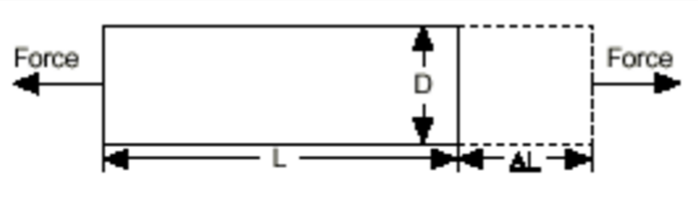
\includegraphics[width=.5\textwidth]{figuras/fig-distension.png}
		\caption{Distension \cite{strain-def}}
		\label{fig:distension}
	\end{figure}

	Generally, the length variation in a strain gauge is very small and this makes them very susceptible to measurement errors. As a result, the use of a Wheatstone bridge is very common, it is formed by four resistive arms and an excitation voltage applied to the bridge \cite{window1982strain}.

	\begin{figure}[htbp]
		\centering
			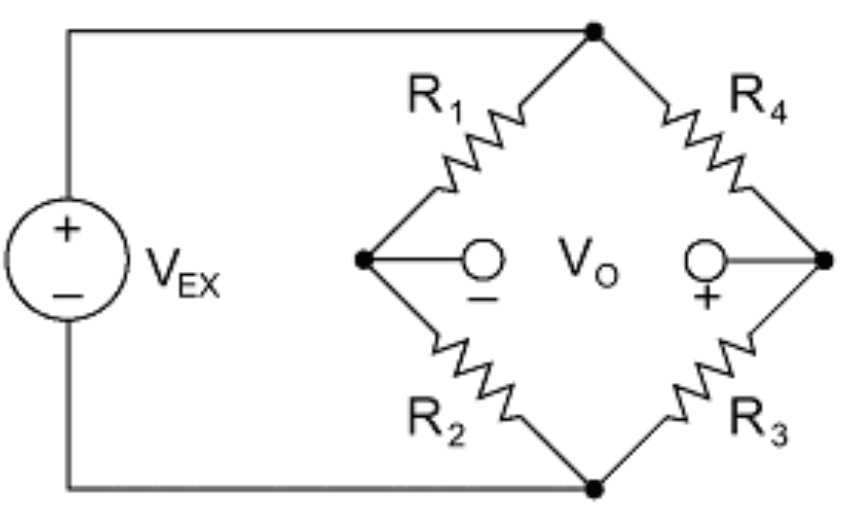
\includegraphics[width=.5\textwidth]{figuras/fig-wheatstone.jpg}
		\caption{Wheatstone bridge \cite{wheat-bridge}}
		\label{fig:wheatstone}
	\end{figure}

	The voltage output $V_{O}$ can be obtained from the Equation \ref{eqn:voWheatstone}, $V_{O}$ \textit{the load cell signal output} is a differential pair signal.

	\begin{equation}\label{eqn:voWheatstone}
		V_{O}=\frac{ R_{3} }{ R_{3} + R_{4} } - \frac{ R_{2} }{ R_{1} + R_{2}}
	\end{equation}

	According to \cite{dillon1989load} the main advantages and drawbacks of Load Cells are: 

	\begin{itemize}
		\item \textit{Accuracy}: usually less than $0.1\%$.\label{itm:accuracy-load-cell}
		\item \textit{Rigid in Construction}: it is extremely resistant to impact and to any mechanical stress.\label{itm:rigid-load-cell}
		\item \textit{Calibration}: load cells are usually already calibrated by manufacturers and vendors.\label{itm:calibration-load-cell}
		\item \textit{Size and Weight}: load cells are bigger and heavier than most force transducers, for applications where size and weight is an important requirement they may not be suitable.\label{itm:size-and-weight}
	\end{itemize}

	Taking all this characteristics into concern the load cell is the most suitable transducer for an automotive test environment.